\documentclass[conference]{IEEEtran}
\IEEEoverridecommandlockouts
% The preceding line is only needed to identify funding in the first footnote. If that is unneeded, please comment it out.
\usepackage{cite}
\usepackage{amsmath,amssymb,amsfonts}
\usepackage{algorithmic}
\usepackage{graphicx}
\usepackage{textcomp}
\usepackage{xcolor}
\def\BibTeX{{\rm B\kern-.05em{\sc i\kern-.025em b}\kern-.08em
T\kern-.1667em\lower.7ex\hbox{E}\kern-.125emX}}
\begin{document}

\title{Energy-Efficient Communication in UAV-assisted Batteryless Wireless Sensor Networks}

\author{
  \IEEEauthorblockN{Miguel Brandt}
  \IEEEauthorblockA{\textit{Department of Informatics} \\
    \textit{Pontifical Catholic University of Rio de Janeiro} \\
    Rio de Janeiro, Brazil \\
  miguelperes@aluno.puc-rio.br}
  \and
  \IEEEauthorblockN{Kelvin Bittencourt}
  \IEEEauthorblockA{\textit{Department of Electrical Engineering} \\
    \textit{Pontifical Catholic University of Rio de Janeiro} \\
    Rio de Janeiro, Brazil \\
  kelvinbitt@gmail.com}
  \and
  \IEEEauthorblockN{Adriano Branco}
  \IEEEauthorblockA{\textit{Department of Informatics} \\
    \textit{Pontifical Catholic University of Rio de Janeiro} \\
    Rio de Janeiro, Brazil \\
  abranco@inf.puc-rio.br}
  \and
  \IEEEauthorblockN{Markus Endler}
  \IEEEauthorblockA{\textit{Department of Informatics} \\
    \textit{Pontifical Catholic University of Rio de Janeiro} \\
    Rio de Janeiro, Brazil \\
  endler@inf.puc-rio.br}
}

\maketitle

\begin{abstract}
  A number of studies have been proposed to tackle the task of monitoring large areas by deploying a wireless sensor network. When communication infrastructure is unavailable, or the region is not easily accessible, data can be retrieved from such networks by using Unmanned Aerial Vehicles (UAVs) as gateways to a base station, thus creating a UAV-assisted Wireless Sensor Network (UAV-WSN).

  However, providing regular maintenance for an extensive, scattered WSN is impractical, leading to devices with limited service life, usually tied to their battery lifespan. Further, they are often treated as disposable, and as a result, become chemical waste.

  In this study, we explore the integration of batteryless sensors powered by energy harvesting (EH) within UAV-WSNs. Since energy-efficient sensors cannot be continuously powered on, we begin by investigating techniques for establishing communication between sensors in a sleep state and UAVs, and ultimately focus on passive wake-up radio receivers, proposing a simple design and discussing the results of real-world experiments.
\end{abstract}

\section{Introduction}

Contexto sobre UAV-WSNs

explicar brevemente EH

aplicacoes

\section{Research scope}

citar gradys

problemas que aparecem ao introduzir EH/intermitencia

focar no problema de wake-up

maybe a diagram showing the full setup

referenciar fig 1 como um cenario

\begin{figure}[htbp]
  \centerline{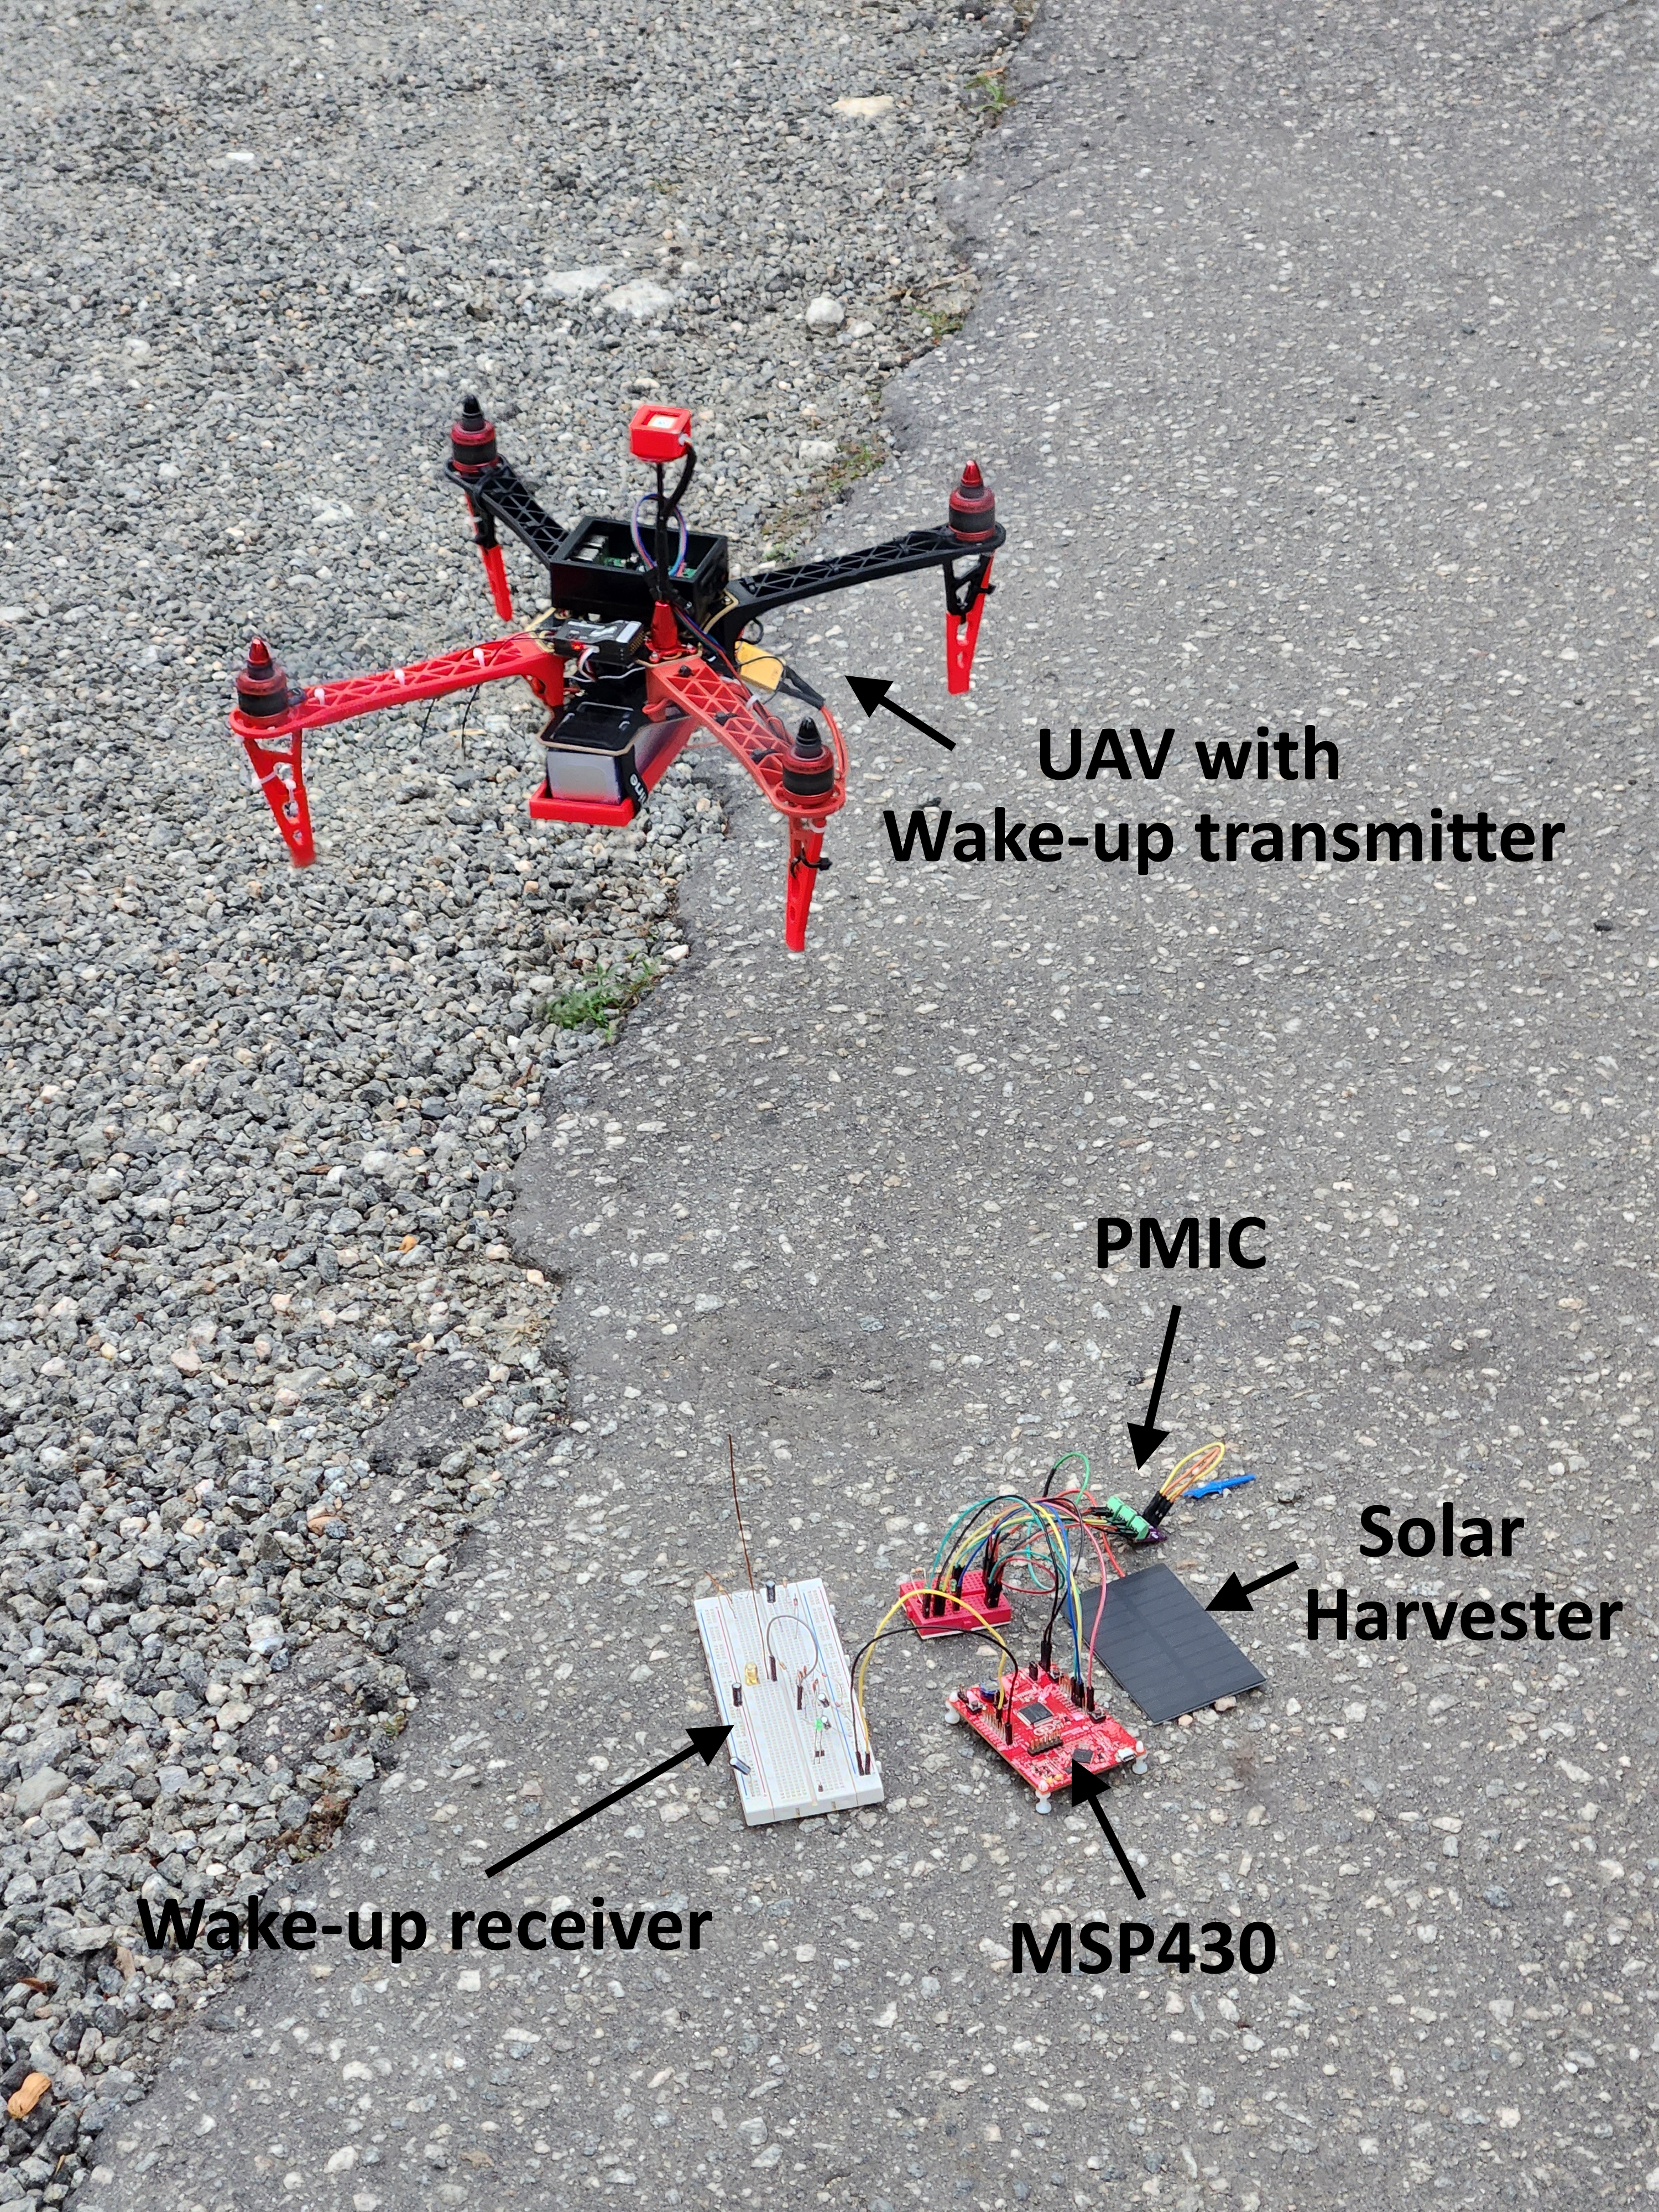
\includegraphics[width=0.8\linewidth]{drone_flying_over_sensor.jpg}}
  \caption{UAV approaching a batteryless sensor to collect data}
  \label{fig:drone_over_sensor}
\end{figure}


\section{Experiment and results}

\subsection{Setup}

In order to conduct experiments, we assembled a passive wake-up radio receiver on a protoboard using off-the-shelf components, based on a voltage doubler circuit, with a 17.3~cm quarter-wave monopole copper wire antenna, as we expect to receive a 433~MHz signal. Since the primary function of the WuRx is to trigger an interrupt in the sensor's GPIO ports, we've also included an 1N4728A voltage clamping Zener diode of 3.3~V to prevent accidental overvoltage on the microcontroller. An LTSpice simulation of the circuit is depicted in Figure \ref{fig:ltspice_receiver}.

In this instance, we performed in-lab measurements with the transmitter powered directly by a DC power supply. The transmitter is a CC1101 radio connected to an ESP32, which is programmed to continuously send a carrier wave with arbitrary data at its maximum power of +12~dBm, in the 433~MHz frequency range. The receiver is connected to an oscilloscope for measuring output voltage, as we hope to achieve at least 2.3~V, which is the minimum threshold for interrupt detection by an MSP430-equipped sensor node.

Although initial tests were performed indoors, we've also built an autonomous, programmable and modular UAV, as seen in Figure \ref{fig:drone_over_sensor}, in order to assess more realistic scenarios.

\subsection{Preliminary findings}

Experiments revealed that the transmitter's output power was unable to charge the receiver's capacitors at a significant rate, except when their antennas were less than 1~cm apart, at which point we attribute the energy transfer to near-field coupling, rather than far-field RF harvesting. Because the UAV cannot hover on top of the receiver for too long, it is essential that the voltage rapidly reaches 2.3~V. Ideally, the UAV would fly over the sensor and collect the necessary data without any deceleration.

To combat this issue, two solutions will be explored: first we will (...)

mention experiments with 433mhz handheld transceiver

mention we want to put an amplifier on the drone, another option would be using harvested energy from the sensor.

\section{Conclusion}

next steps

want to conduct outdoors tests with the drone, amplifier mounted, measure motor interference

optimize energy transfer: investigate better antenna designs, dipole antenna option ignores ground plane

\bibliographystyle{IEEEtran}
\bibliography{references}

\end{document}
